\documentclass[10pt]{article}

\usepackage[spanish,mexico]{babel}
\usepackage[utf8]{inputenc}
\usepackage{apacite}

\usepackage{anysize}
\marginsize{2cm}{2cm}{2cm}{2cm}
\setlength{\parskip}{8px}

\usepackage{hyperref}

\usepackage{amsmath}
\usepackage{amssymb}
\usepackage{amsfonts}
\usepackage{cancel}

\usepackage{graphicx}
\usepackage{float}

\usepackage{caption}
\usepackage{subcaption}

\usepackage{xcolor}

\usepackage{fancyhdr}

\usepackage{listings}

\usepackage{longtable}
\usepackage{colortbl}
\usepackage{diagbox}
\usepackage{tabularx}

\usepackage{tcolorbox}


\newcolumntype{L}[1]{>{\hsize=#1\hsize\raggedright\arraybackslash}X}%
\newcolumntype{R}[1]{>{\hsize=#1\hsize\raggedleft\arraybackslash}X}%
\newcolumntype{C}[2]{>{\hsize=#1\hsize\columncolor{#2}\centering\arraybackslash}X}%

\renewcommand{\tabularxcolumn}[1]{m{#1}}

\pagestyle{fancy}
\fancyhf{}
\rhead{3CM19}
\lhead{Computing Selected Topics}
\cfoot{\thepage}
\renewcommand{\footrulewidth}{0.4pt}

\definecolor{blueTitle}{rgb}{0.05,0.31,0.48}
\definecolor{blueSub}{rgb}{0.95,0.97,0.98}
\definecolor{blue}{rgb}{0.4, 0.6, 0.8}

\newcommand{\HRule}{\textcolor{blueTitle}{\rule{\linewidth}{0.5mm}}}

\begin{document}

    \thispagestyle{empty}

    \begin{center}
        \begin{minipage}{0.48\textwidth}
            \begin{flushleft}
                \hspace{1cm}
\includegraphics[width=1.5cm]{ipn.png}
            \end{flushleft}
        \end{minipage}
        \begin{minipage} {0.48\textwidth}
            \begin{flushright}
                
\includegraphics[width=2.7cm]{escom.png}
            \end{flushright}
        \end{minipage}

        \vspace*{-2cm}

        \LARGE
        \textcolor{blueTitle}{\textbf{Instituto Politécnico Nacional\\}}
        \LARGE
        \textcolor{blueTitle}{Escuela Superior de Cómputo}

        \vspace{2cm}
        
        \Large
        \textbf{Computing Selected Topics} \\
        \vspace{.3cm}
        Sistemas Complejos
        \vspace{1.5cm}
        
        \Large
        \textbf{Profesor} \\
        \vspace{.3cm}
        Genaro Juárez Martínez
        \vspace{1cm}
        
        \HRule
        \vspace{.4cm}
        {\textbf{Práctica 2} \smallskip
        
        La Hormiga de Langton}
        \HRule
        \vspace{1.5cm}

        \Large
        \textbf{Alumno} \\
        \vspace{.3cm}
       
        Reyes Rodríguez Enrique Abdiel\\
        \vspace{.3cm}
        \vspace{1cm}

        \Large
        \textbf{Grupo} \\
        \vspace{.3cm}
        3CM19
        \vspace{1cm}

    \end{center}
    
    \newpage
    \tableofcontents
    \newpage
    \section{Objetivo general}
        		En esta práctica se aborda la creación de un Autómata Celular o por sus siglas en ingles (AC) llamado la Hormiga de Langton, nuestro objetivo es poder generar dicho autómata con sus reglas y poder visualizar como este va comportando y evolucionando.

    \section{Introducción}
Como ya se mencionado anteriormente, un autómata celular es un modelo matemático para un sistema dinámico, este sistema evoluciona con el paso del tiempo. El autómata celular está compuesto por un conjunto células o celdas las cuales adquieren distintos valores o estados. Al ser este un sistema dinámico y al evolucionar a través del tiempo estos estados o valores que poseen las células son alterados de un instante a otro en un tiempo discreto, es decir, conocemos que valores toman nuestras células o celda en un cierto punto en el tiempo, en otras palabras es posible hacer una cuantización.
Siendo así, el conjunto de células evolucionan según la expresión matemática, la cual evolucionará según los estados de las células vecinas, a esto se le conoce como regla de transición local.

	\section{Elementos de un AC}
		\subsection{Un espacio rectangular}
		El autómata celular está definido ya sea en un espacio de dos dimensiones o bien en un espacio de n dimensiones, este es el espacio de evoluciones y cada una de las divisiones de este espacio es llamada célula.
		
		\subsection{Conjunto de estados}
		Los estados son finitos y cada elemento de la célula tomará un valor de este conjunto de estados. A cada vecindad diferente le corresponde un elemento del conjunto de estados.
 	
		\subsection{Configuración inicial o tiempo 0}
		Es la asignación inicial de un estado a cada una de las células del espacio.		
		
		\subsection{Función local o Función de transición local}
		Es la regla de evolución que determina el comportamiento del autómata celular. Esta regla esta conformada por una célula central y sus vecindades. También esta define como debe cambiar de estado cada una de las células dependiendo de los estados de las vecindades anteriores. Esta función puede ser representada como una función algebraica o como un conjunto de ecuaciones. 
        
	
	\section{Clasificación de los Autómatas Celulares}
	Stephen Wolfram comenzó a trabajar en autómatas celulares a mediados de 1981 después de considerar cómo los patrones complejos parecían formarse en la naturaleza en violación de la segunda ley de la termodinámica. Sus investigaciones fueron inicialmente impulsados por un interés en sistemas de modelado, como las redes neuronales. Tras ver la inesperada complejidad del comportamiento de estas reglas simples Wolfram llevó a sospechar que la complejidad en la naturaleza puede ser debida a mecanismos similares. En 2002 Wolfram publicó su libro A New Kind of Science, que sostiene ampliamente que los descubrimientos sobre autómatas celulares no son hechos aislados sino que son robustos y tienen importancia para todas las disciplinas de la ciencia. 

	Wolfram define cuatro clases en las que los AC. Mientras que los estudios anteriores en autómatas celulares tienden a tratar de identificar el tipo de patrones de reglas específicas, la clasificación de Wolfram fue el primer intento de clasificación global. En orden de complejidad las clases que identifica son:
		
		\subsection{Clase I}
		Casi todos los patrones iniciales evolucionan rápidamente en un estado estable y homogéneo. Cualquier aleatoriedad en el patrón inicial desaparece.
			
		\subsection{Clase II}
		Casi todos los patrones iniciales evolucionan rápidamente hacia estructuras estables u oscilantes. Parte de la aleatoriedad del patrón inicial puede permanecer, pero solo algunos restos. Los cambios locales en el patrón inicial tienden a permanecer locales.
			
		\subsection{Clase III} 
		Casi todos los patrones iniciales evolucionan de forma pseudo-aleatoria o caótica. Las estructuras estables que aparecen son destruidas rápidamente por el ruido circundante. Los cambios locales en el patrón inicial tienden a propagarse indefinidamente.
			
		\subsection{Clase IV}
		Casi todos los patrones iniciales evolucionan en las estructuras que interactúan de manera compleja e interesante, con la formación de las estructuras locales que son capaces de sobrevivir por largos períodos de tiempo. Podría ser el caso de que apareciesen estructuras estables u oscilantes, pero el número de pasos necesarios para llegar a este estado puede ser muy grande, incluso cuando el patrón inicial es relativamente simple. Los cambios locales en el patrón inicial pueden extenderse indefinidamente. Wolfram ha conjeturado que muchos, si no todos, los AC de esta clase son capaces de realizar computación universal. Algo que ha sido demostrado para el juego de la vida de John Conway.
    \section{La Hormiga de Langton}
        La hormiga de Langton es un autómata celular diseñado por Chris Langton en 1986. Es un autómata celular que en si es una máquina de Turing también, por lo cual se pueden realizar algoritmos computables. La existencia de la máquina en el AC fue demostrada hasta el año 2000. Se le considera un sistema de Turing completo ya que puede simular cualquier máquina de Turing, siendo este clasificado como autómata celular de Clase IV.
        \subsection{Las reglas}
            La evolución de este está regida por el estado inicial y no necesita entrada alguna posteriormente. El mapa donde las células evolucionaran es una matriz de un tamaño definido.  El juego evoluciona a partir de unidades de tiempo discretas (iteraciones). El estado de todas las celulas se tiene en cuenta para calcular el estado de las mismas en el turno siguiente.
            Cada cuadrado del entramado se colorea o bien blanco o bien negro. Se identifica arbitrariamente un cuadrado como la «hormiga». La hormiga siempre está mirando en una de las cuatro direcciones cardinales y se mueve un cuadrado cada vez, de acuerdo con las siguientes reglas:
            \begin{itemize}
                \item Si está sobre un cuadrado blanco, cambia el color del cuadrado, gira noventa grados a la izquierda y avanza un cuadrado.
                \item Si está sobre un cuadrado negro, cambia el color del cuadrado, gira noventa grados a la derecha y avanza un cuadrado.
            \end{itemize}
		
        

    
    \section{Programa}	
		\subsection{Descripción}
        Este programa se realizó con la tecnología de Python (pygame, matplotlib, numpy). Las limitaciones en las especificaciones de la computadora en donde se ejecutó provocan que la ejecución con dimensiones arriba de 500x500 sean muy lentas, por lo que las pruebas se harán con un tamaño de 35X70.
        \subsection*{Controles}
            \begin{itemize}
                \item r: reiniciar mapa
                \item g: llenar mapa con hormigas aleatorias
                \item mouse click : coloca una hormiga en la posicion indicada
                \item p: genera la grafica de densidad poblacional
                \item s: guarda un archivo con los datos del mapa
                \item l: carga un archivo con los datos del mapa
                \item k: borra la ultima hormiga insertada
            \end{itemize}
        \subsection*{Evolución}
        En la hormiga de Lanton, su población se puede analizar de maneras distintas, por ejemplo:
            \subsubsection{Decesos por aislamiento}
            En este caso, la población del sistema decae por la baja reproducción dado que no hay interacción entre hormigas reinas y reproductoras.
              \begin{figure}[h!]
                \centering
                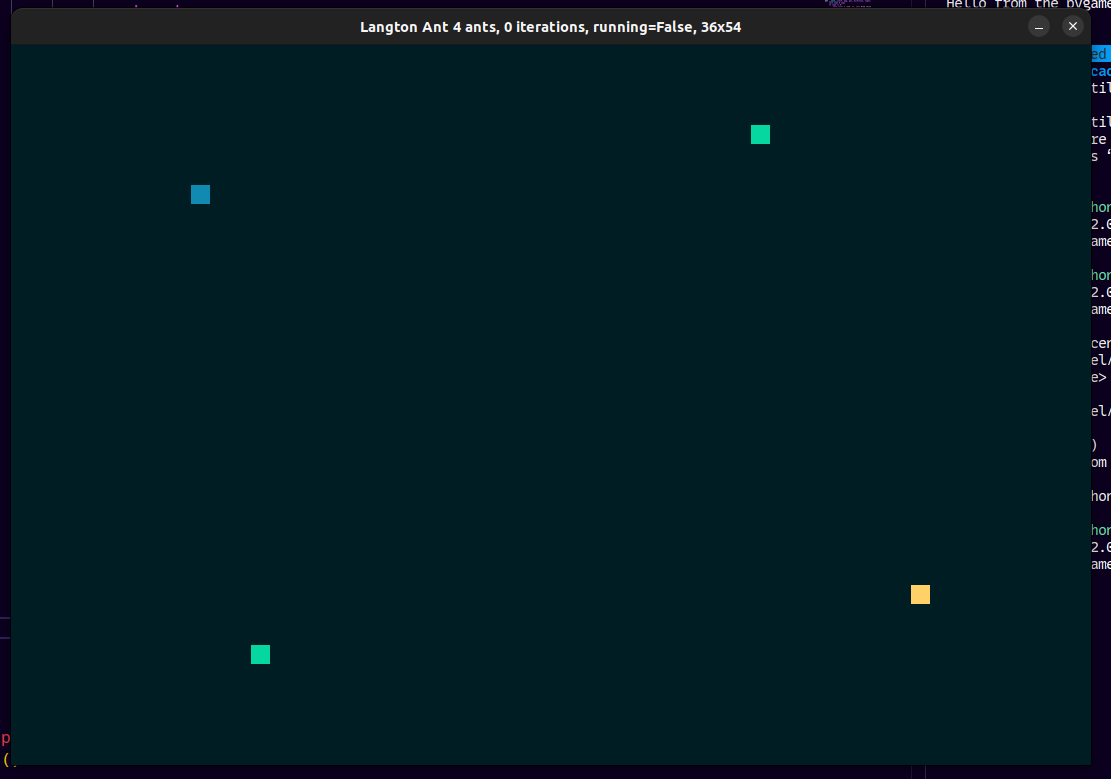
\includegraphics[width=0.5\textwidth]{aislamiento1.png}
            \end{figure}\begin{figure}[h!]
                \centering
                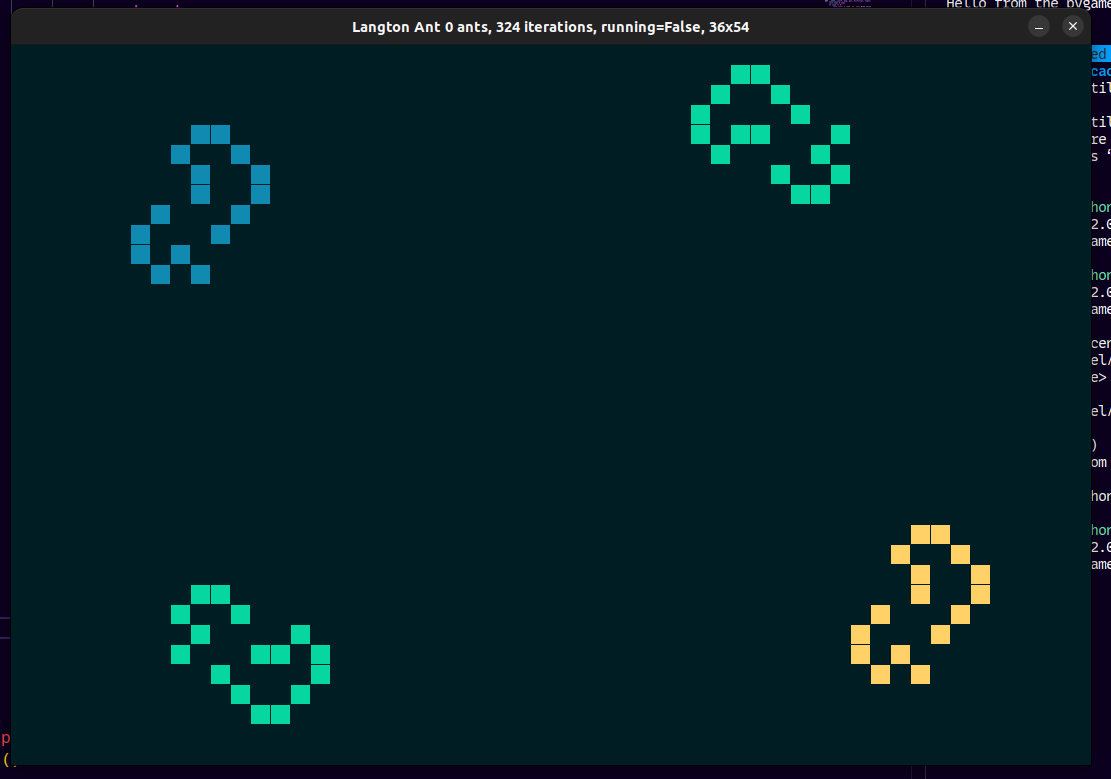
\includegraphics[width=0.5\textwidth]{aislamiento2.png}
            \end{figure}\begin{figure}[h!]
                \centering
                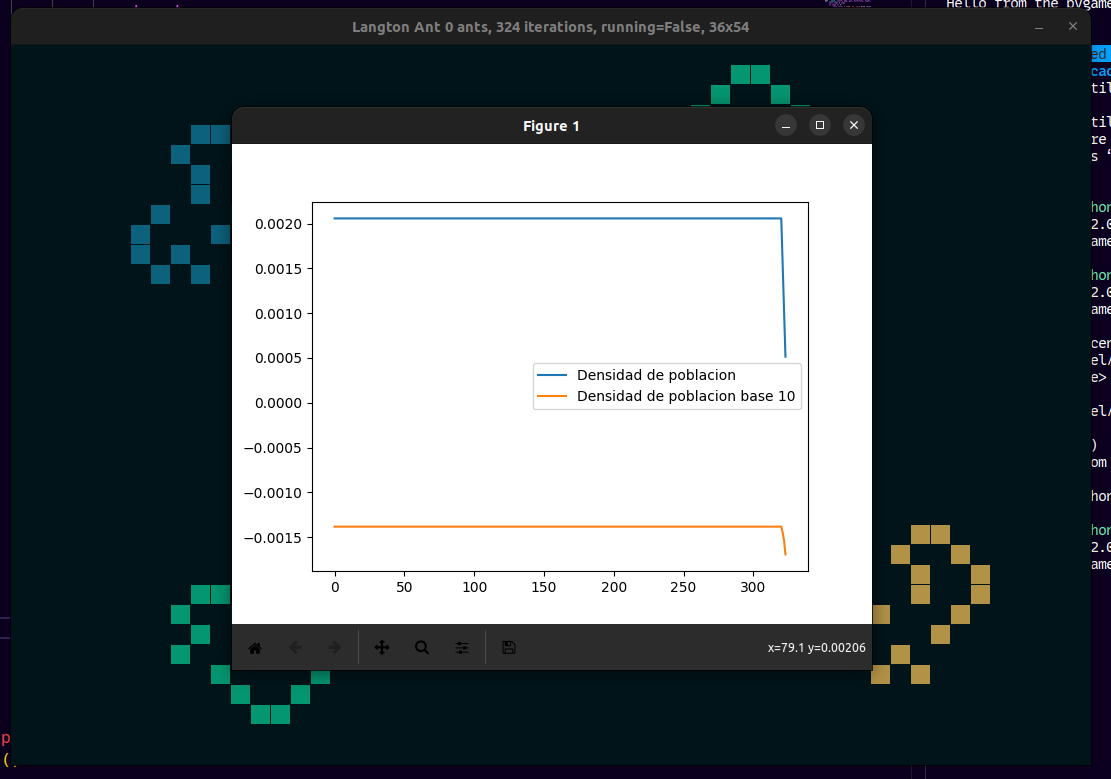
\includegraphics[width=0.5\textwidth]{aislamiento3.png}
            \end{figure}
            \subsubsection{Decesos por sobrepoblación}
            En este caso, la población del sistema decae por el exceso de hormigas nuevas que no cumplen con las condiciones de reproducción
            \begin{figure}[h!]
                \centering
                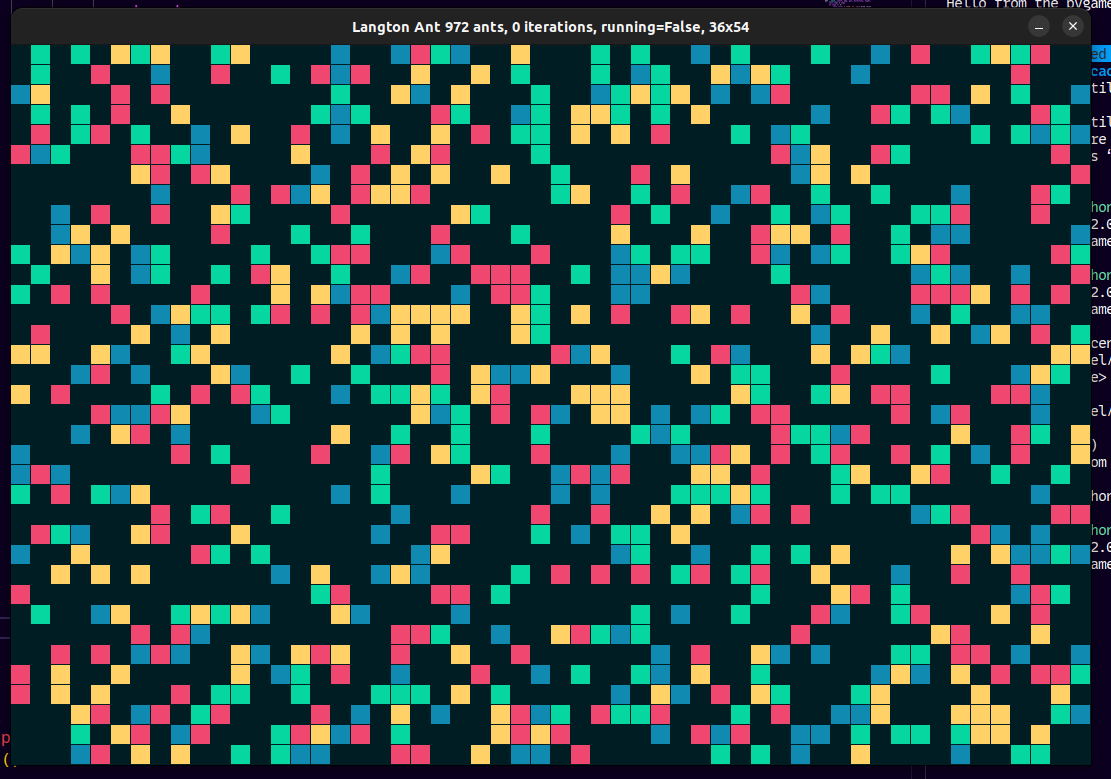
\includegraphics[width=0.5\textwidth]{sobrepoblacion1.png}
            \end{figure}
            \begin{figure}[h!]
                \centering
                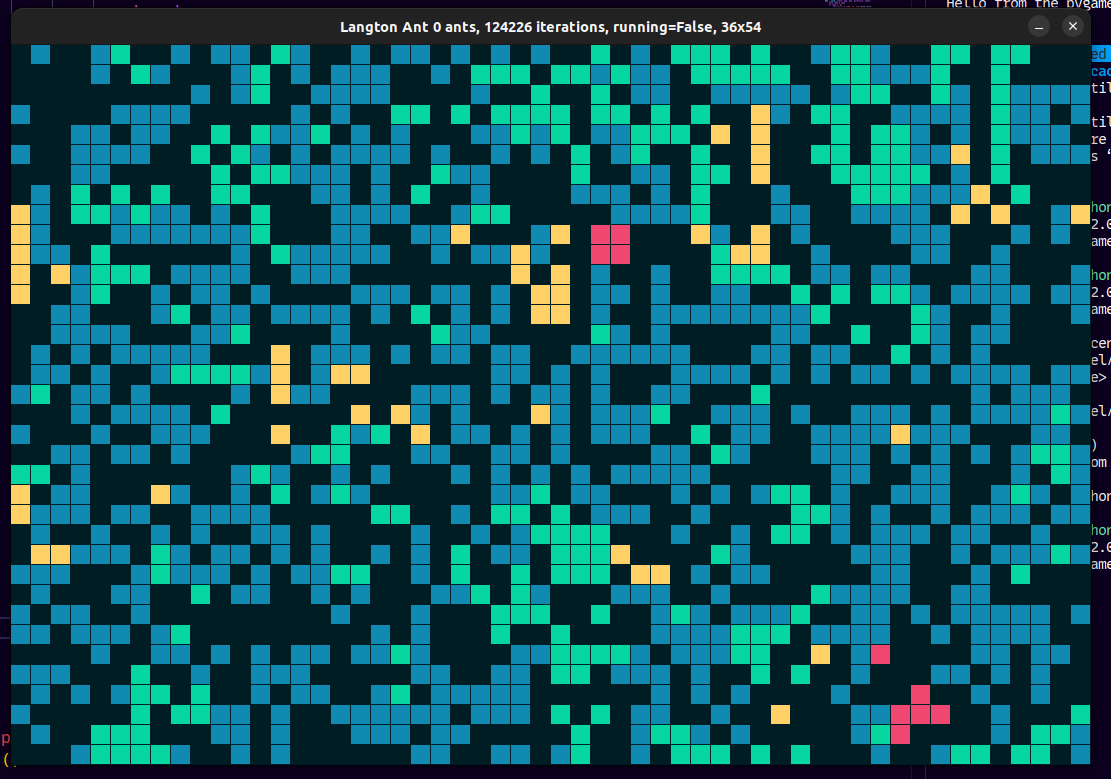
\includegraphics[width=0.5\textwidth]{sobrepoblacion2.png}
            \end{figure}
            \begin{figure}[h!]
                \centering
                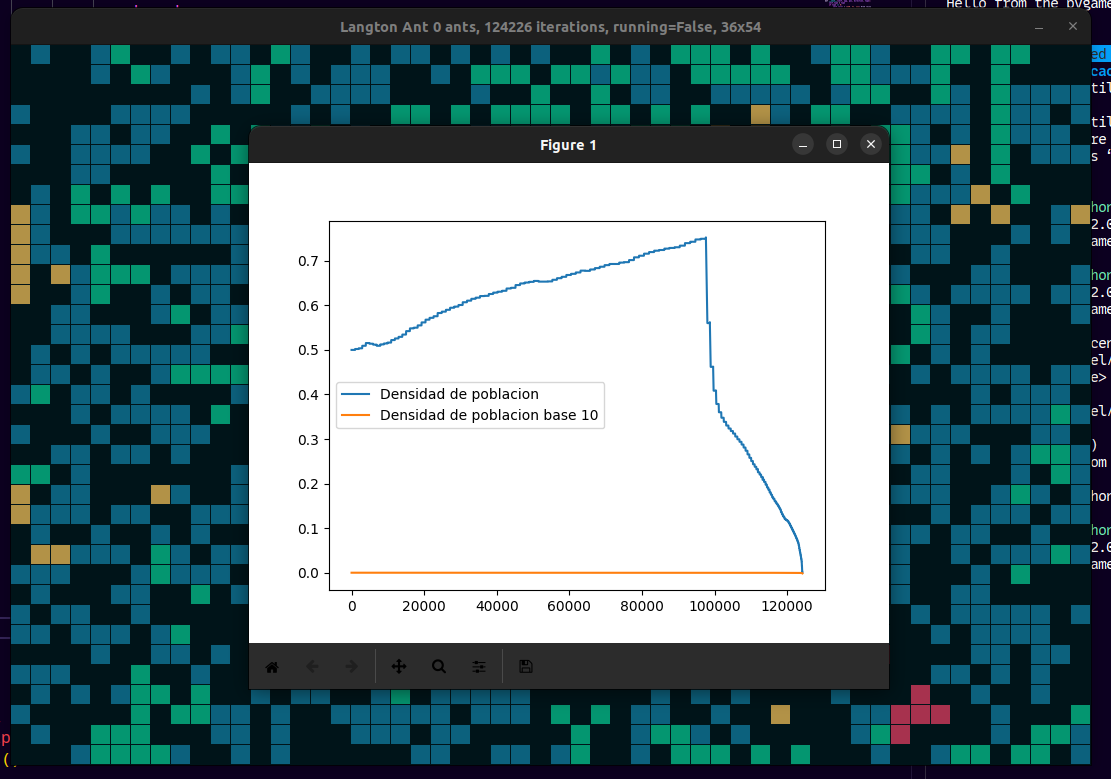
\includegraphics[width=0.5\textwidth]{sobrepoblacion3.png}
            \end{figure}
            \subsubsection{Sistema estable}
            En este caso, la poblacion del sistema se mantiene estable por un gran numero de iteraciones.
            \begin{figure}[h!]
                \centering
                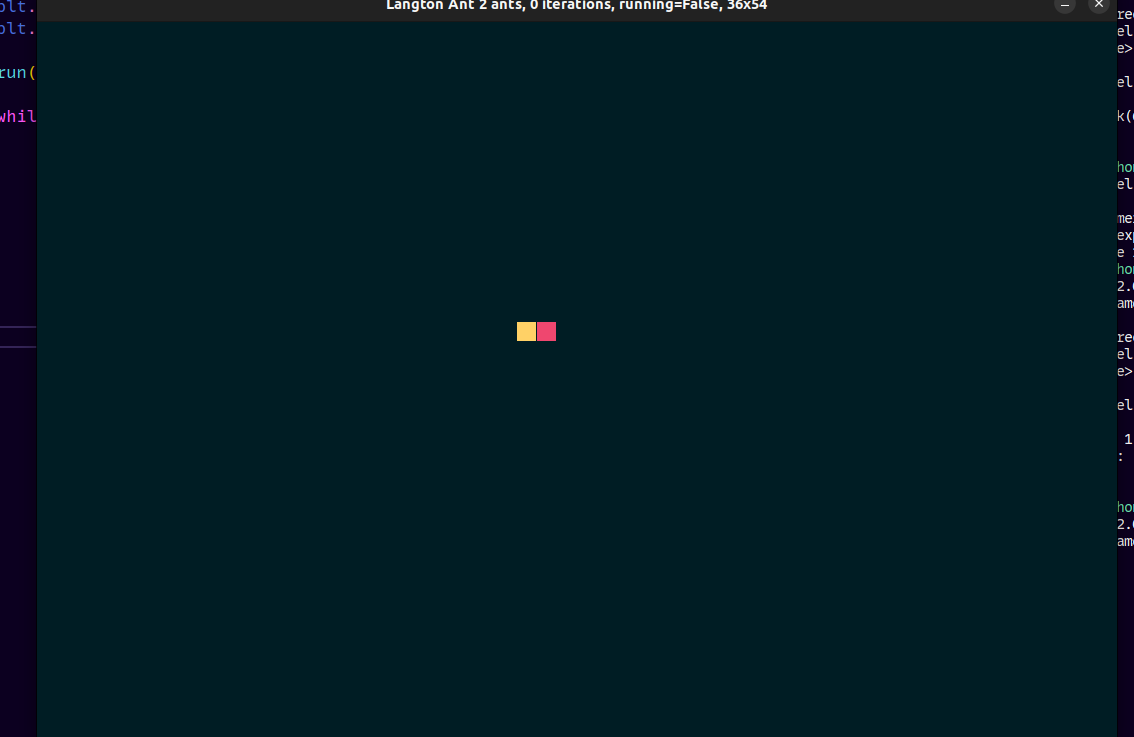
\includegraphics[width=0.5\textwidth]{estable1.png}
            \end{figure}
            \begin{figure}[h!]
                \centering
                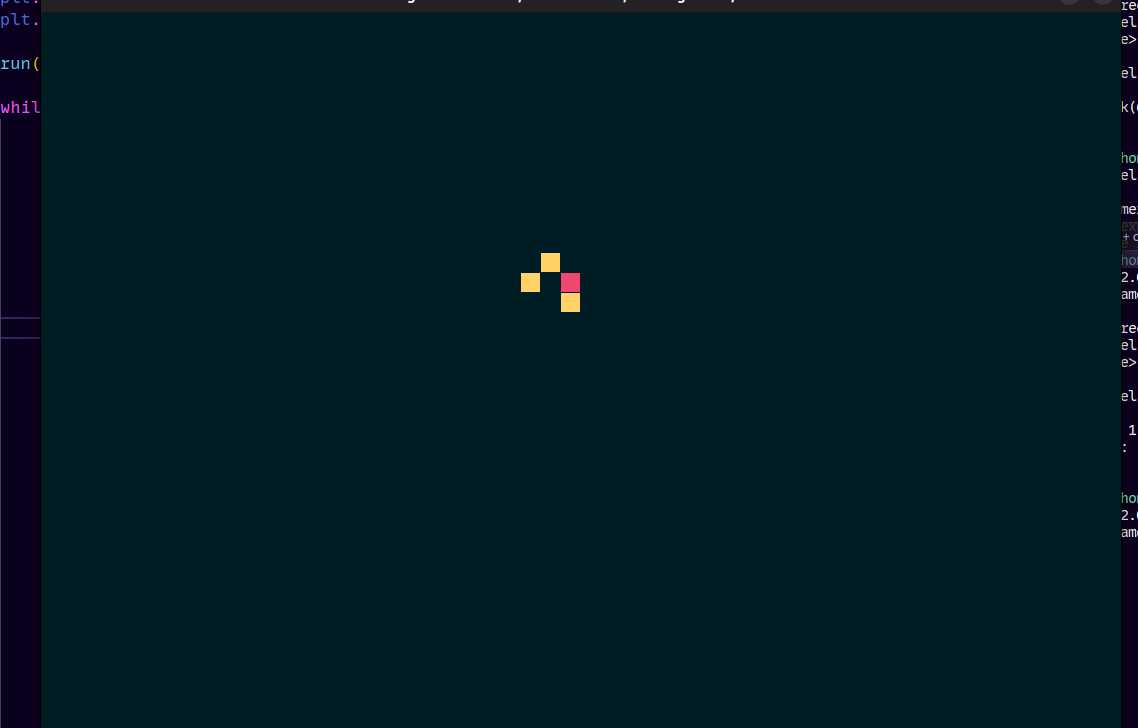
\includegraphics[width=0.5\textwidth]{estable2.png}
            \end{figure}
            \begin{figure}[h!]
                \centering
                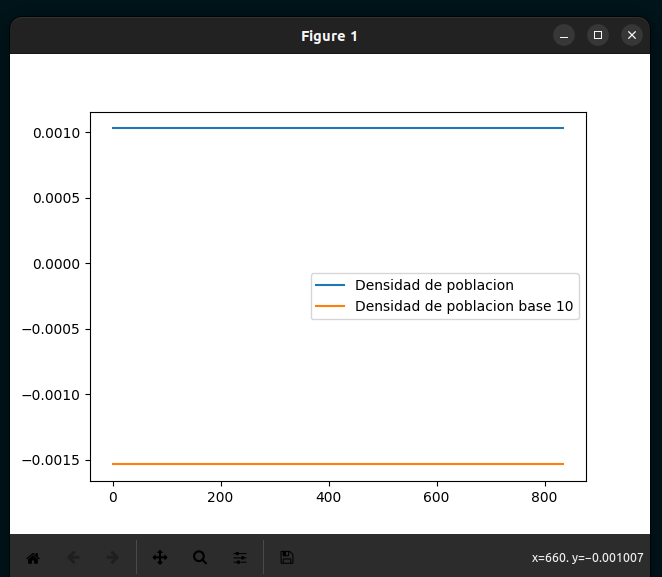
\includegraphics[width=0.5\textwidth]{estable3.png}
            \end{figure}
        \newpage
        \subsection{Código}
            El programa es un archivo, el cual tiene 2 clases principales, App y Ant. App se encarga de administrar la ventana y el mapa, mientras Ant es el automata celular que actualiza su posición en el mapa y se dibuja.  
            \subsubsection{main.py}
            \lstset{language=Python}
                \begin{verbatim}

import pygame as pg
from collections import deque
from random import choice, randrange
import numpy as np
import pickle
import time
import datetime
import tkinter as tk
from  tkinter import filedialog
from pprint import pprint
import matplotlib.pyplot as plt
black = (0, 29, 36)
class Ant:
    def __init__(self, app, pos, direction, type):
        self.type = type
        if type == 0:
            self.color = (239, 71, 111) #red reina
        if type == 1:
            self.color = (255, 209, 102) #yellow reproductora
        if type == 2:
            self.color = (6, 214, 160) #green trabajador
        if type == 3:
            self.color = (17, 138, 178) #blue soldado
        self.x, self.y = pos
        self.life = 0
        #para rotar la hormiga, solo cambiamos la posicion[0] de increments al final del array
        #y asi se va rotando entre las direcciones
        self.increments = deque([(1, 0), (0, 1), (-1, 0), (0, -1)])
        self.increments.rotate(direction)

    def run(self,app):
        value = app.grid[self.y][self.x]
        #cambiamos el valor de una celda ocupada/desocupada en el mapa
        app.grid[self.y][self.x] = not value

        SIZE = app.CELL_SIZE
        rect = self.x * SIZE, self.y * SIZE, SIZE - 1, SIZE - 1
        if value:
            pg.draw.rect(app.screen, pg.Color(black), rect)
        else:
            pg.draw.rect(app.screen, self.color, rect)
        #por hormiga, recorremos las direcciones
        self.increments.rotate(1) if value else self.increments.rotate(-1)
        dx, dy = self.increments[0]
        self.x = (self.x + dx) % app.COLS
        self.y = (self.y + dy) % app.ROWS
        self.life += 1


class App:
    def __init__(self, WIDTH=1080, HEIGHT=720, CELL_SIZE=20):
        pg.init()
        self.screen = pg.display.set_mode([WIDTH, HEIGHT])
        self.clock = pg.time.Clock()
        self.screen.fill(black)
        self.CELL_SIZE = CELL_SIZE
        self.ROWS, self.COLS = HEIGHT // CELL_SIZE, WIDTH // CELL_SIZE
        self.grid = [[0 for col in range(self.COLS)] for row in range(self.ROWS)]
        self.ants = []
        self.running = False
        self.iterations = 0
        self.plot_pop = []
    def generate_random_ants(self):
        for i in range(int(self.COLS*self.ROWS/2)):
            direction = np.random.randint(0,4)
            type = np.random.randint(0,4)
            c,r = randrange(self.COLS), randrange(self.ROWS)
            rect = c * self.CELL_SIZE, r * self.CELL_SIZE, self.CELL_SIZE - 1, self.CELL_SIZE - 1
            a = Ant(self, (c,r), direction, 
            type)
            pg.draw.rect(self.screen, a.color, rect)
            self.ants.append(a)
    def generate_ant(self,x,y):
        direction = np.random.randint(0,4)
        type = np.random.randint(0,100)
        if(type<=1):
            type = 0 #1%
        elif(type <= 9):
            type = 1 #9%
        elif(type<=35):
            type = 2 #35%
        else:
            type = 3 #55%
        a = Ant(self, (x,y), direction, 
        type)
        rect = x * self.CELL_SIZE, y * self.CELL_SIZE, self.CELL_SIZE - 1, self.CELL_SIZE - 1
        pg.draw.rect(self.screen, a.color, rect)
        self.ants.append(a) 
    def create_mouse_ant(self):
        mx,my = int(pg.mouse.get_pos()[0]/self.CELL_SIZE), int(pg.mouse.get_pos()[1]/self.CELL_SIZE)
        value = self.grid[my][mx]
        self.grid[my][mx] = not value
        rect = mx * self.CELL_SIZE, my * self.CELL_SIZE, self.CELL_SIZE - 1, self.CELL_SIZE - 1
        if value:
            pg.draw.rect(self.screen, pg.Color(black), rect)
            self.ants.pop()
        else:
            self.generate_ant(mx,my)
    def get_grid_values(self,x,y):
        if x >= self.ROWS:
            x -= self.ROWS
        elif x < 0:
            x += self.ROWS
        if y >= self.COLS:
            y -= self.COLS
        elif y < 0:
            y += self.COLS
        return self.grid[x][y]
    def graph(self,b : list,s:int):
        s = np.array(s)
        population = np.divide(np.array(b),s)
        populationlog = np.divide(np.log10(population),s)
        plt.plot(population,label="Densidad de poblacion")
        plt.plot(populationlog, label="Densidad de poblacion base 10")
        plt.legend()
        plt.show()
    
    def run(self):
        
        while True:
            #actualizamos mapa
            if(self.running):
                for i,a in enumerate(self.ants):
                    if(self.running):
                        a.run(app=self)
                        self.iterations += 1
                        
                        self.plot_pop.append(len(self.ants))
                        if a.life > 80:
                            del self.ants[i]
            #analizamos colisiones
                for i,a in enumerate(self.ants):
                    for abc in self.ants[:-i]:
                        x,y = abc.x, abc.y
                        if ((x-a.x) == 1 or (x-a.x) == 1) and ((y-a.y) == 1 or (y-a.y) == 1):
                            if abc.type == 0 and a.type == 1:
                                #nace hormiga
                                self.generate_ant(a.x,a.y)
                            if abc.type == 0 and a.type == 0:
                                #pelea reinas
                                if abc.life == a.life:
                                    survive = np.random.randint(0,2)
                                    if survive == 1:
                                        if self.ants.count(a) >0 : self.ants.remove(a)
                                        if self.ants.count(abc) > 0:self.ants.remove(abc)
                                    

            for i in pg.event.get():
                if i.type == pg.QUIT:
                    exit()
                if i.type == pg.KEYDOWN:
                    if i.key == pg.K_SPACE:
                        self.running = not self.running
                    if i.key == pg.K_r:
                        self.__init__()
                        break
                    if i.key == pg.K_g:
                        self.generate_random_ants()
                    if i.key == pg.K_k:
                        self.ants.pop()
                    if i.key == pg.K_s:
                        a = [self.grid,self.ants]
                        with open(f'langton_{self.COLS}_{self.ROWS}_{int(time.mktime(datetime.datetime.now().timetuple()))}.ant', 'wb') as f:
                            pickle.dump(a,f)
                    if i.key == pg.K_l:
                        file_path = filedialog.askopenfilename(filetypes=(
                        ("Ant Files","*.ant"),
                        ("All Files", "*.*")
                        ))
                        print(file_path)
                        if file_path != "":
                            with open(file_path, 'rb') as f:
                                data = pickle.load(f)
                                self.grid = data[0]
                                self.ants = data[1]
                                [ant.run(app=self) for ant in self.ants]
                    if i.key == pg.K_p and (not self.running):
                        self.graph(self.plot_pop,int(self.COLS*self.ROWS))
                if i.type == pg.MOUSEBUTTONDOWN:
                    self.create_mouse_ant()                   
            pg.display.flip()
            pg.display.set_caption(f'Langton Ant {len(self.ants)} ants, {self.iterations} iterations, running={self.running}')
            self.clock.tick(60)


if __name__ == '__main__':
    app = App()
    app.run()
                \end{verbatim}
    
    
    \section{Conclusiones}
    Hubieron muchas cosas interesantes en la realización de la práctica, empezando en la forma de abordar el problema. Uno pensaría que con matrices sería suficiente, pero la complejidad temporal y espacial se eleva mucho, sobretodo al analizar los nacimientos y peleas. Esta práctica demostró de manera excelente el comportamiento de los autómatas celulares. Ya que la hormiga de Langton evoluciona mucho dependiendo de el numero de hormigas en el mapa, se observaba también que al cambiar las restricciones (como el tiempo de vida y las condiciones de nacimiento), el comportamiento variaba mucho, siendo mas ordenado, o incluso más caótico. 
    \bibliographystyle{apacite}
    \begin{thebibliography}{1}
        \bibitem[1]{c0}Weisstein, E., 2021. Elementary Cellular Automaton. Recuperado 15 de enero de 2023, de \url{https://mathworld.wolfram.com/ElementaryCellularAutomaton.html}
        \bibitem[2]{c1} Caparrini, F. S. Autómatas Celulares - Fernando Sancho Caparrini. Recuperado 15 de enero de 2023, de \url{http://www.cs.us.es/%7Efsancho/?e=66}
        \bibitem[3]{c2} colaboradores de Wikipedia. Recuperado 15 enero de 2023. Hormiga de Langton. Wikipedia, la enciclopedia libre \url{https://es.wikipedia.org/wiki/Hormiga_de_Langton}
    \end{thebibliography}
    
\end{document}